\cohead{\Large\textbf{Verhältnis von Flächen}}
\fakesubsection{Verhältnis von Flächen}
\begin{tcolorbox}
	\textbf{Verhältnis von Flächen:}\\
	\textcolor{loestc}{Das Verhältnis zweier Flächen lässt sich bestimmen, indem man die beiden Flächen durcheinander teilt, z.B. stehen die beiden Flächen \(A_1=2\) und \(A_2=4\) im Verhältnis \(1:2\), da \(\dfrac{A_1}{A_2}=\dfrac{1}{2}\) gilt.
	}
\end{tcolorbox}
\begin{minipage}{\textwidth}
	\begin{minipage}{.6\textwidth}\raggedright
		Beispiele:\\
		Zeige, dass die Gerade \textcolor{blue}{\(g(x)=-x\)} die von der \(x\)-Achse und der Funktion \textcolor{red}{\(f(x)=x^2-4x\)} eingeschlossene Fläche \(A\) im Verhältnis \(27:37\) teilt:\\
		\textcolor{loes}{Die zwei Teilflächen lassen sich z.B. wie folgt bestimmen:}
		\textcolor{loes}{Fläche zwischen \(f(x)\) und der \(x\)-Achse:}.\\
		\textcolor{loes}{\(\displaystyle A=-\int_0^4 x^2-4x \td x=\frac{32}{3}\)}
		\textcolor{loes}{Fläche zwischen \(f(x)\) und \(g(x)\):}.\\
		\textcolor{loes}{\(\displaystyle A_1=\int_0^3 -x-\left(x^2-4x\right) \td x=\frac{9}{2}\)}\\		
		\textcolor{loes}{Die Fläche, die von der \(x\)-Achse und den beiden Funktionen eingeschlossen wird, beträgt also \(A_2=A-A_1=\tfrac{37}{6}\)}.\\
		\textcolor{loes}{Damit teilt die Gerade die Fläche \(A\) im Verhältnis \(\dfrac{A_1}{A_2}=\dfrac{27}{37}\)}.\\
	\end{minipage}
	\begin{minipage}{.4\textwidth}
		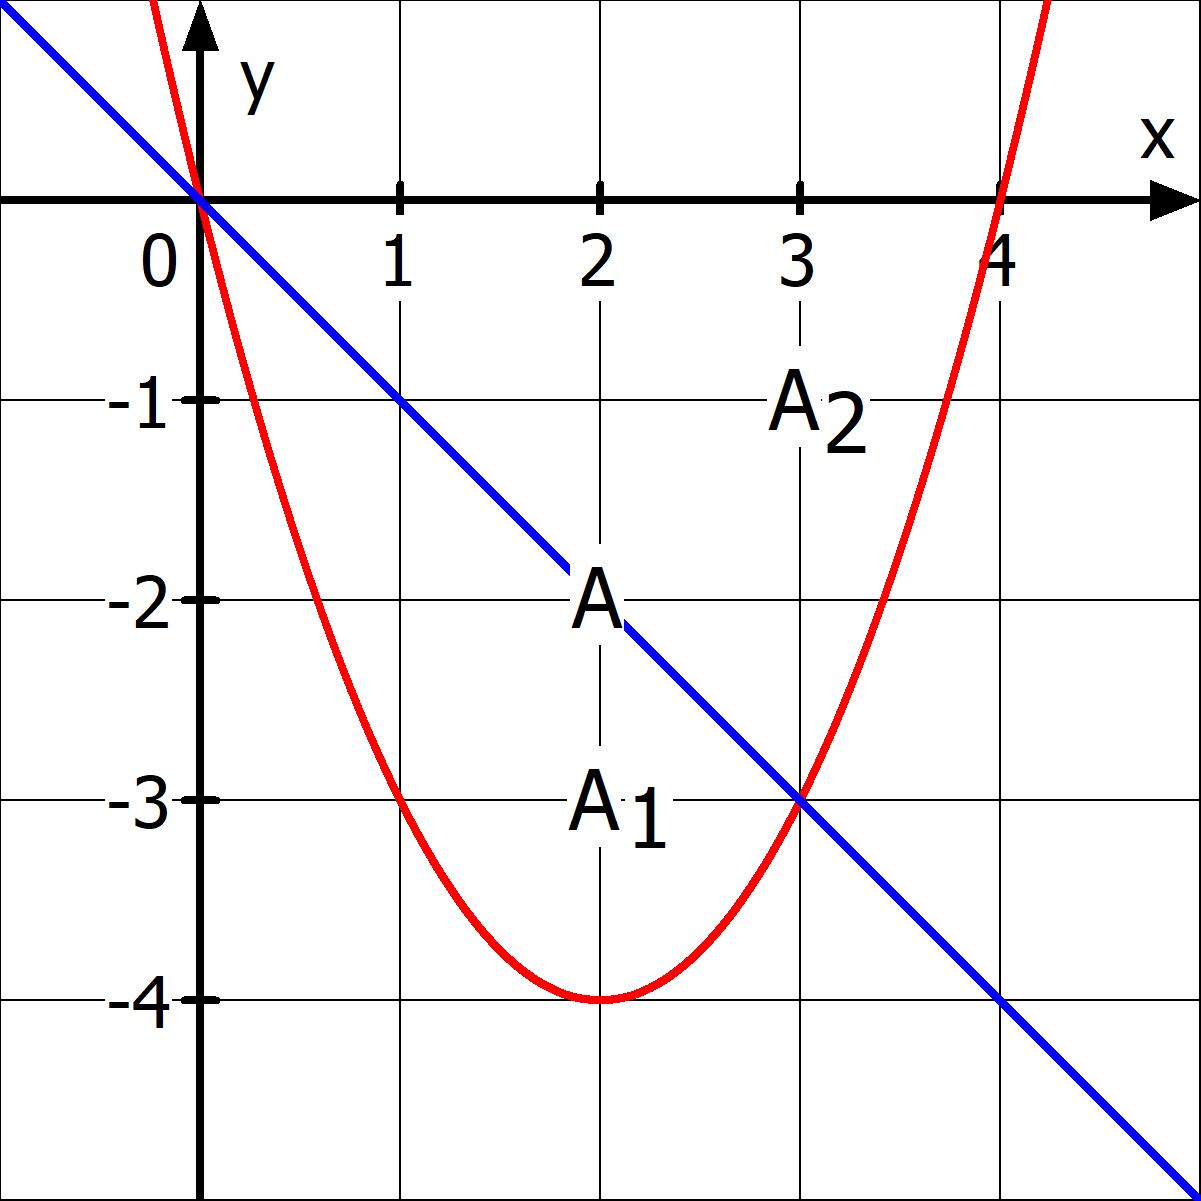
\includegraphics[width=.95\linewidth]{\integration/pics/VerhaeltnisBsp1.png}
	\end{minipage}
\end{minipage}\vspace{\baselineskip}\\
\begin{minipage}{\textwidth}
	\begin{minipage}{.4\textwidth}
		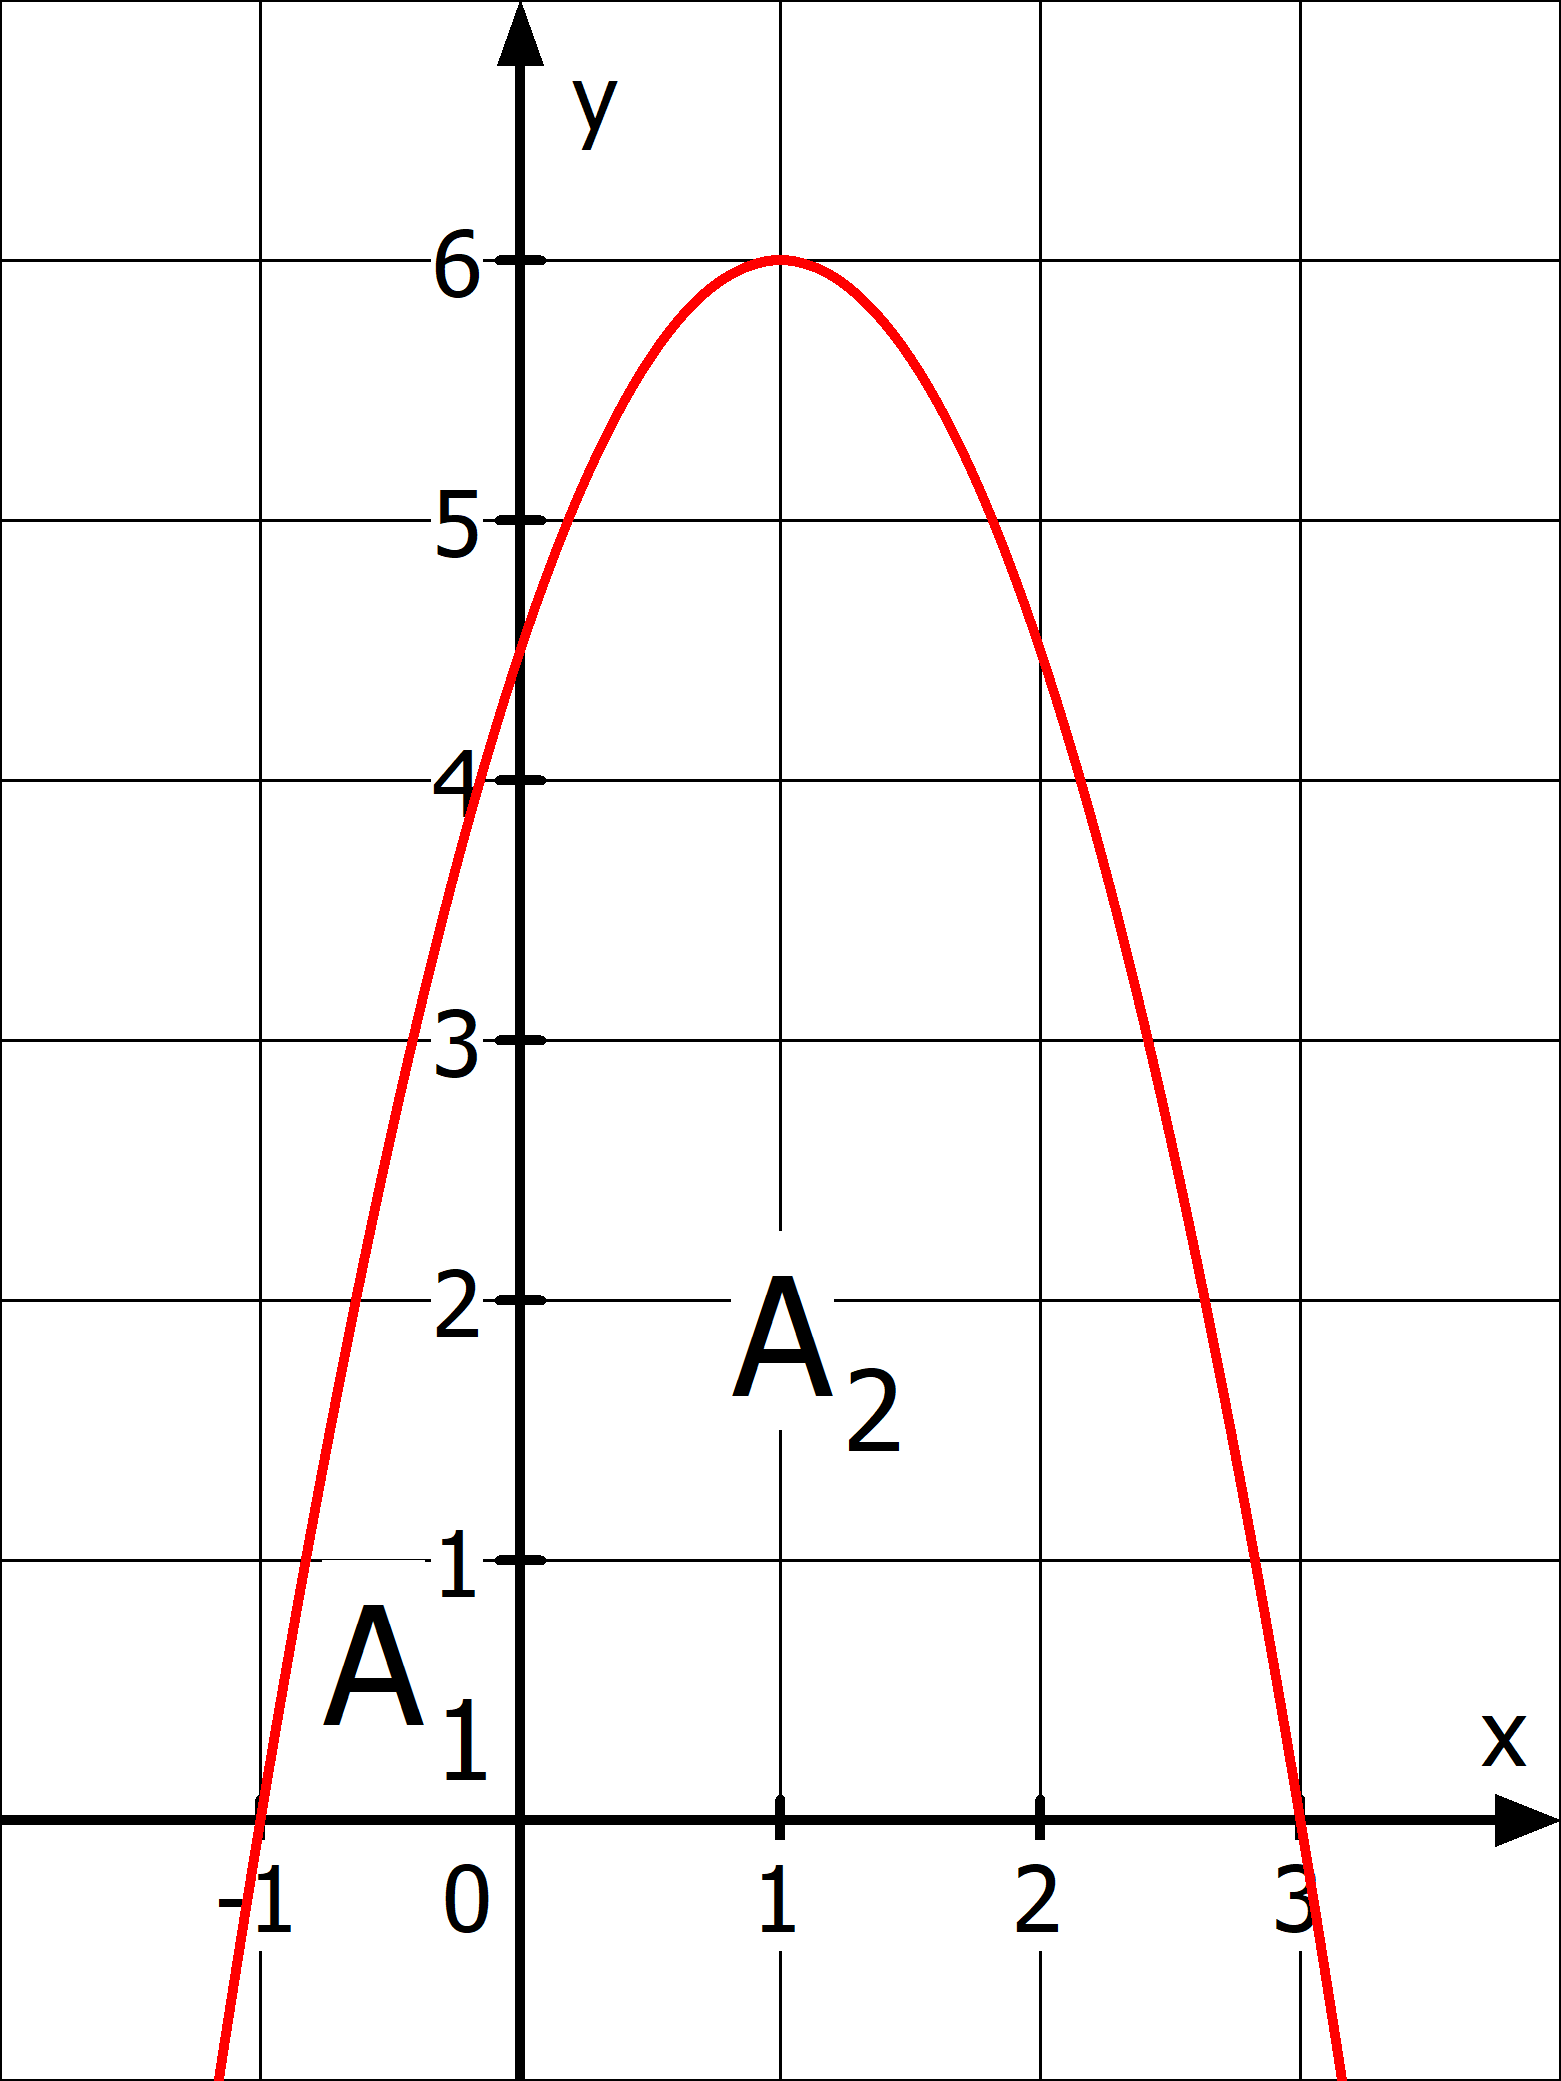
\includegraphics[width=.95\linewidth]{\integration/pics/VerhaeltnisBsp2.png}
	\end{minipage}
	\begin{minipage}{.6\textwidth}\raggedright
		Bestimme in welchem Verhältnis die \(y\)-Achse die von \textcolor{red}{\(f(x)=-1,5x^2+3x+4,5\)} und der \(x-\)Achse eingeschlossenen Fläche teilt.\\
		\textcolor{loes}{Die zwei Teilflächen lassen sich z.B. wie folgt bestimmen:}\\
		\textcolor{loes}{Flächeninhalt der linken der beiden Teilflächen:}.\\
		\textcolor{loes}{\(\displaystyle A_1=-\int_{-1}^0 -1,5x^2+3x+4,5 \td x=\frac{5}{2}\)}\\
		\textcolor{loes}{Flächeninhalt der rechten der beiden Teilflächen:}.\\
		\textcolor{loes}{\(\displaystyle A_2=-\int_0^3 -1,5x^2+3x+4,5 \td x=\frac{27}{2}\)}\\
		\textcolor{loes}{Damit teilt die \(y\)-Achse die Fläche zwischen der Funktion und der \(x\)-Achse im Verhältnis \(\dfrac{A_1}{A_2}=\dfrac{5}{27}\)}.\\
	\end{minipage}
\end{minipage}\vspace{\baselineskip}\\
\newpage

\begin{Exercise}[title={\raggedright\normalfont Gegeben sind die Gerade \(x=1\) und die Funktion \(f(x)=-\frac{1}{2}x^2+3x\), ihr Schaubild sei \(K_f\) Die Fläche \(A\) sei die von \(K_f\) und der \(x\)-Achse eingeschlossene Fläche.}, label=verhaltnisFlaechenA1]
	\begin{enumerate}[label=\alph*)]
		\item Zeichne \(K_f\) und die Gerade \(x=1\) in ein Koordinatensystem.
		\item Zeige, dass die Gerade \(x=1\) die Fläche \(A\) im Verhältnis 2:25 teilt.
	\end{enumerate}
\end{Exercise}

\begin{Exercise}[title={\raggedright\normalfont Gegeben sind die Funktion \(g(x)=\frac{1}{6}x^3+\frac{1}{2}x^2\) und ihr Schaubild \(K_g\).}, label=verhaltnisFlaechenA2]\\
	\begin{minipage}{\textwidth}
		\begin{minipage}{.6\textwidth}
			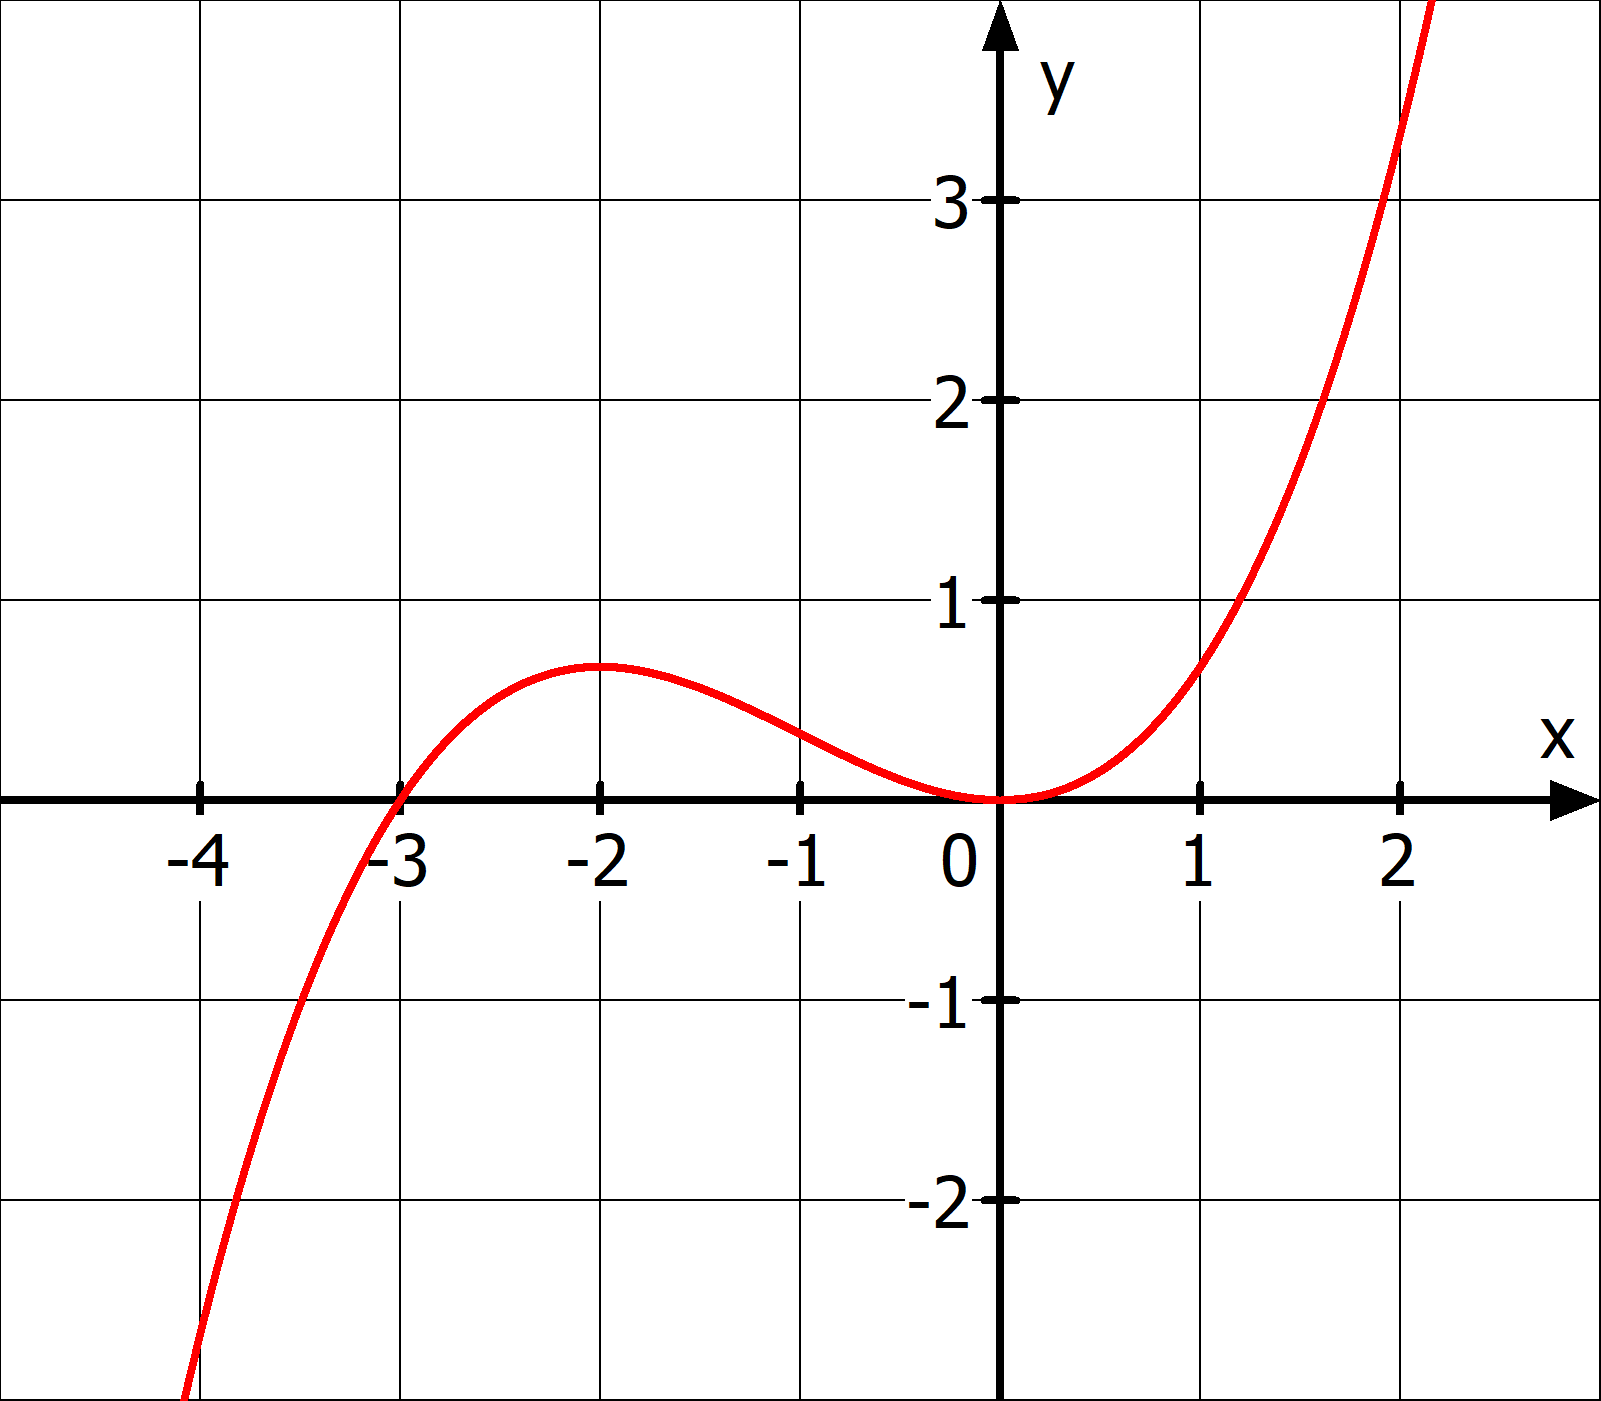
\includegraphics[width=.95\linewidth]{\integration/pics/VerhaeltnisAuf2.png}
		\end{minipage}
		\begin{minipage}{.4\textwidth}\raggedright
			\begin{enumerate}[label=\alph*)]
				\item \(K_g\), die \(x\)-Achse und die Gerade \(x=-4\) schließen 2 Flächen ein. Zeige, dass diese gleich groß sind.
				\item \(K_g\), die \(x\)-Achse und die Gerade \(x=2\) schließen 2 Flächen ein. Zeige, dass diese im Verhältnis 16:9 stehen.		
			\end{enumerate}
		\end{minipage}
	\end{minipage}
\end{Exercise}

\begin{Exercise}[title={\raggedright\normalfont Gegeben sind die Funktion \(h(x)=-\frac{1}{18}x^3+\frac{1}{2}x^2\) und ihr Schaubild \(K_h\).}, label=verhaltnisFlaechenA3]\\
	\begin{minipage}{\textwidth}
		\begin{minipage}{.4\textwidth}\raggedright
			\begin{enumerate}[label=\alph*)]
				\item Zeige, dass die von \(K_h\) und der \(x\)-Achse eingeschlossene Fläche \(A\) den Flächeninhalt \(\frac{243}{8}\) hat.
				\item Zeichne die Gerade \(i(x)=-\frac{1}{2}x+\frac{9}{2}\) ein. Der Schnittpunkt der Geraden \(i(x)\) mit \(K_h\) ist \(S(3\vert 3)\).\\
				Zeige, dass die Gerade die Fläche \(A\) im Verhältnis 16:11 teilt.					
			\end{enumerate}
		\end{minipage}
		\begin{minipage}{.6\textwidth}
			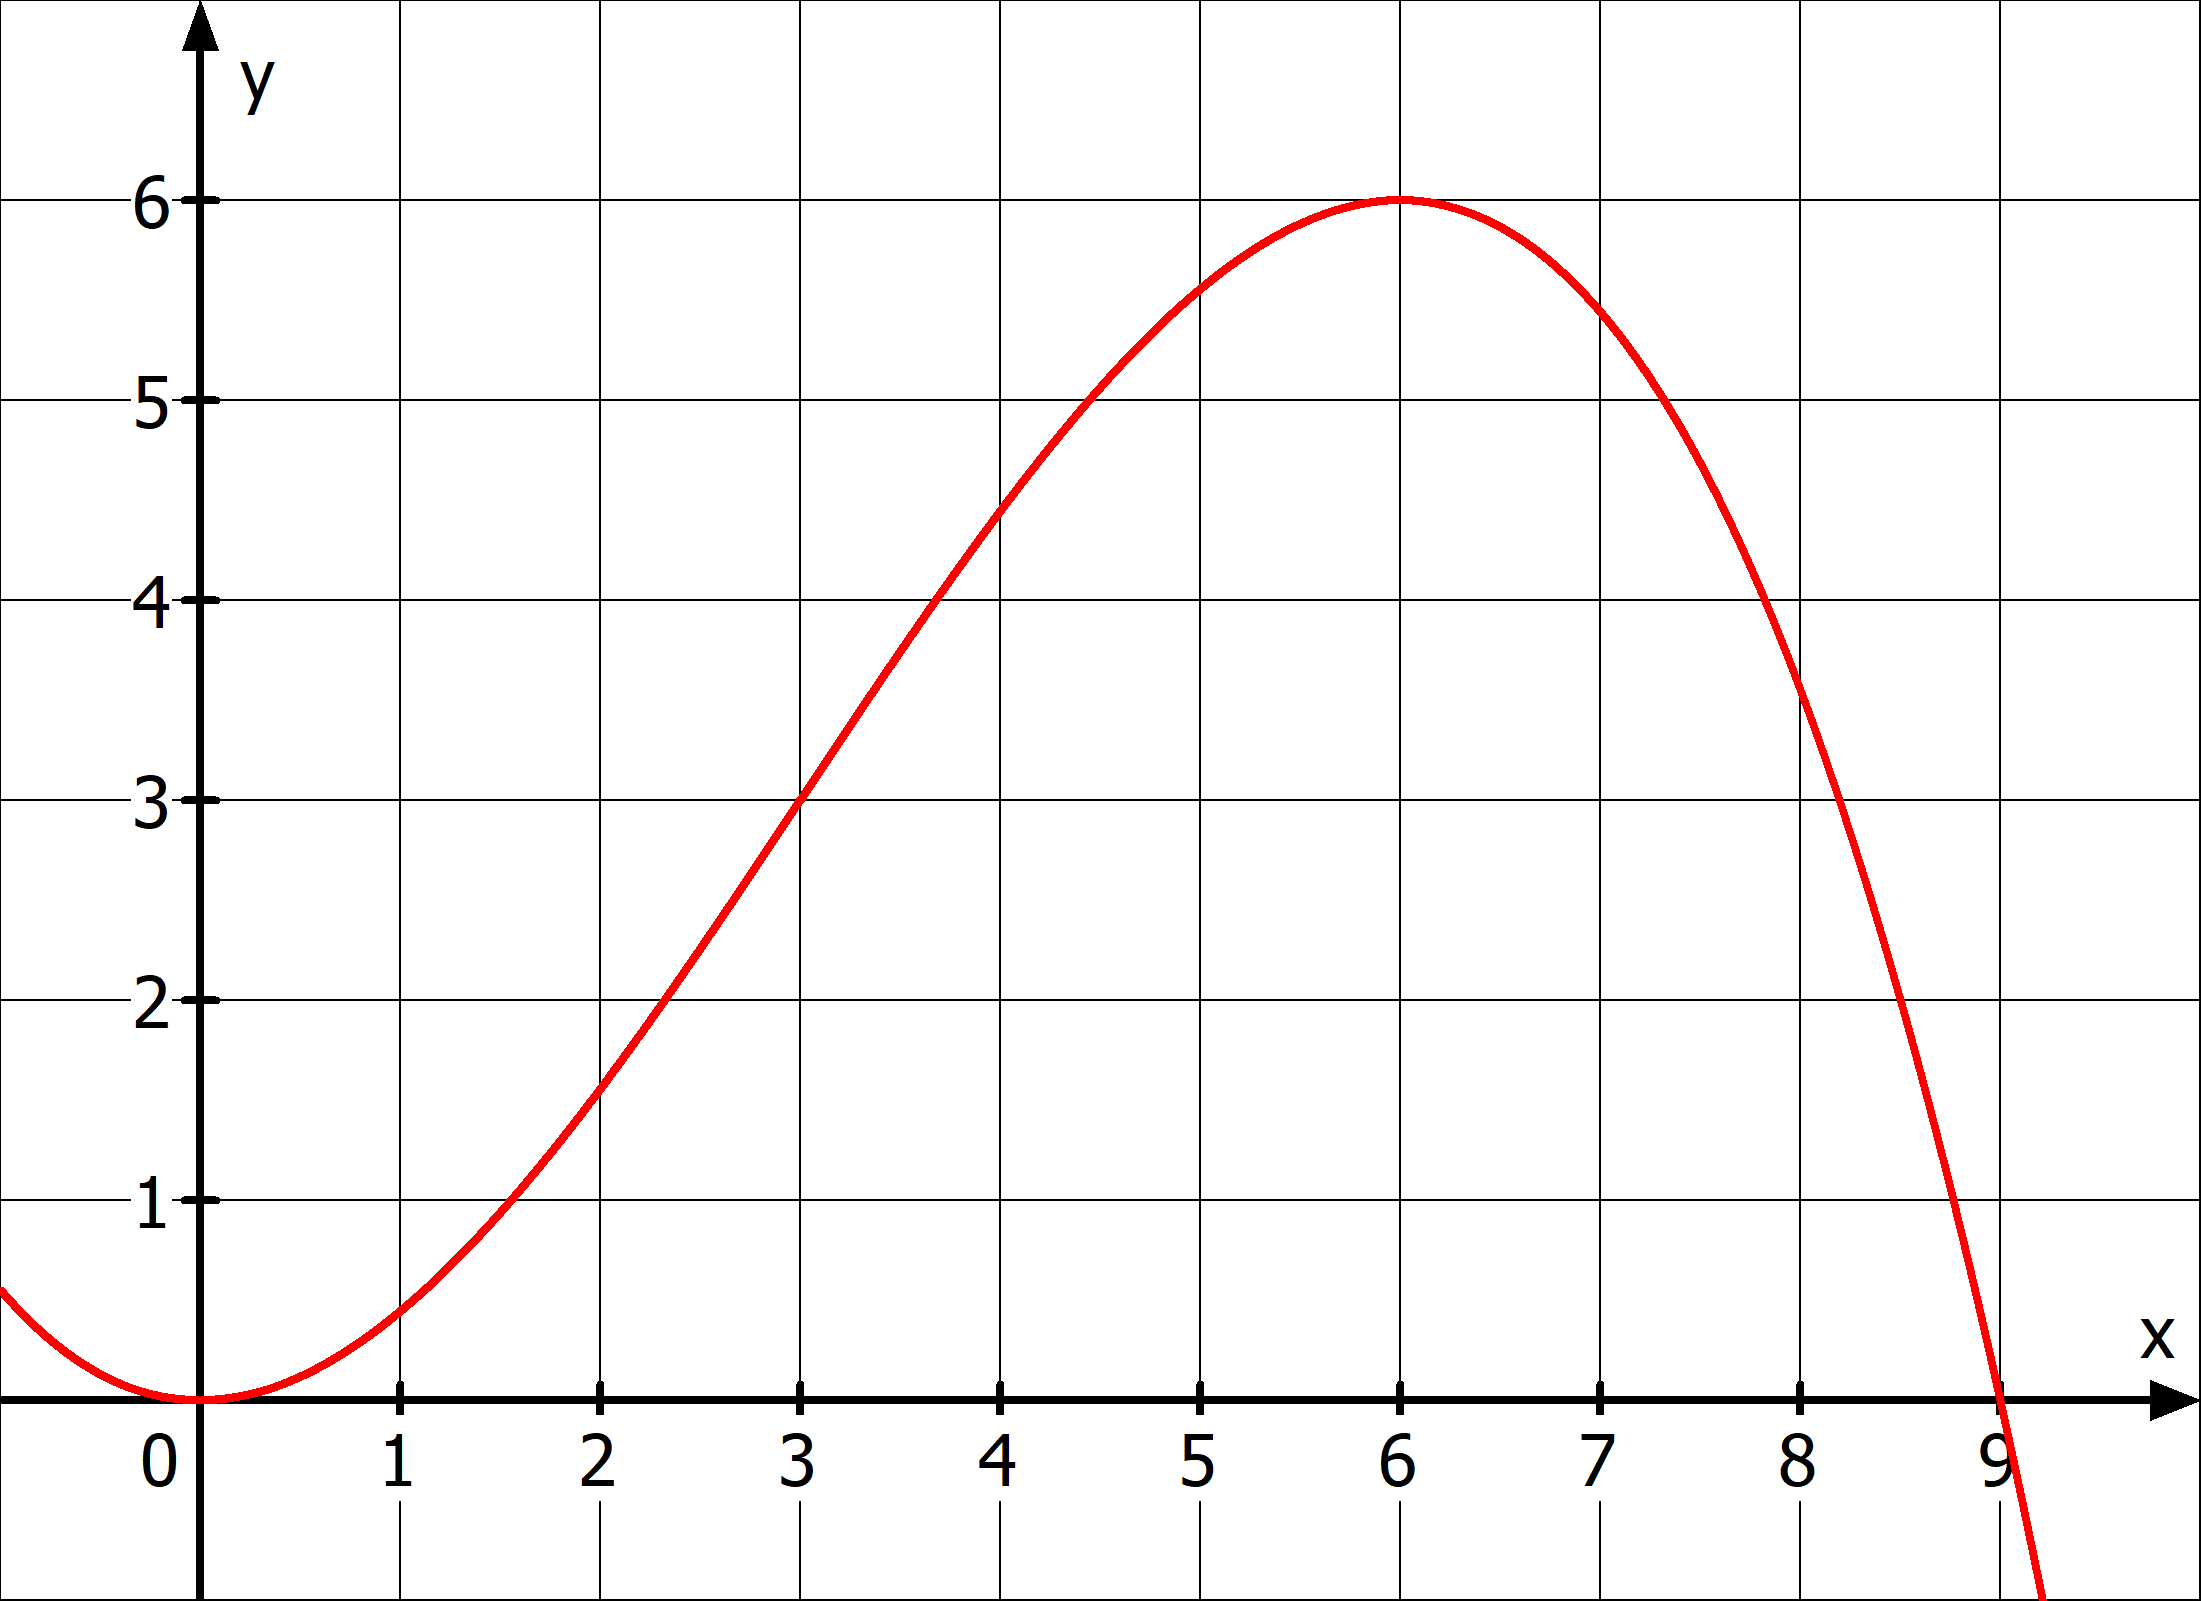
\includegraphics[width=.95\linewidth]{\integration/pics/VerhaeltnisAuf3.png}
		\end{minipage}
	\end{minipage}
\end{Exercise}

%%%%%%%%%%%%%%%%%%%%%%%%%%%%%%%%%%%%%%%%%
\begin{Answer}[ref=verhaltnisFlaechenA1]\\
	\begin{minipage}{\textwidth}
		\begin{minipage}{.4\textwidth}
			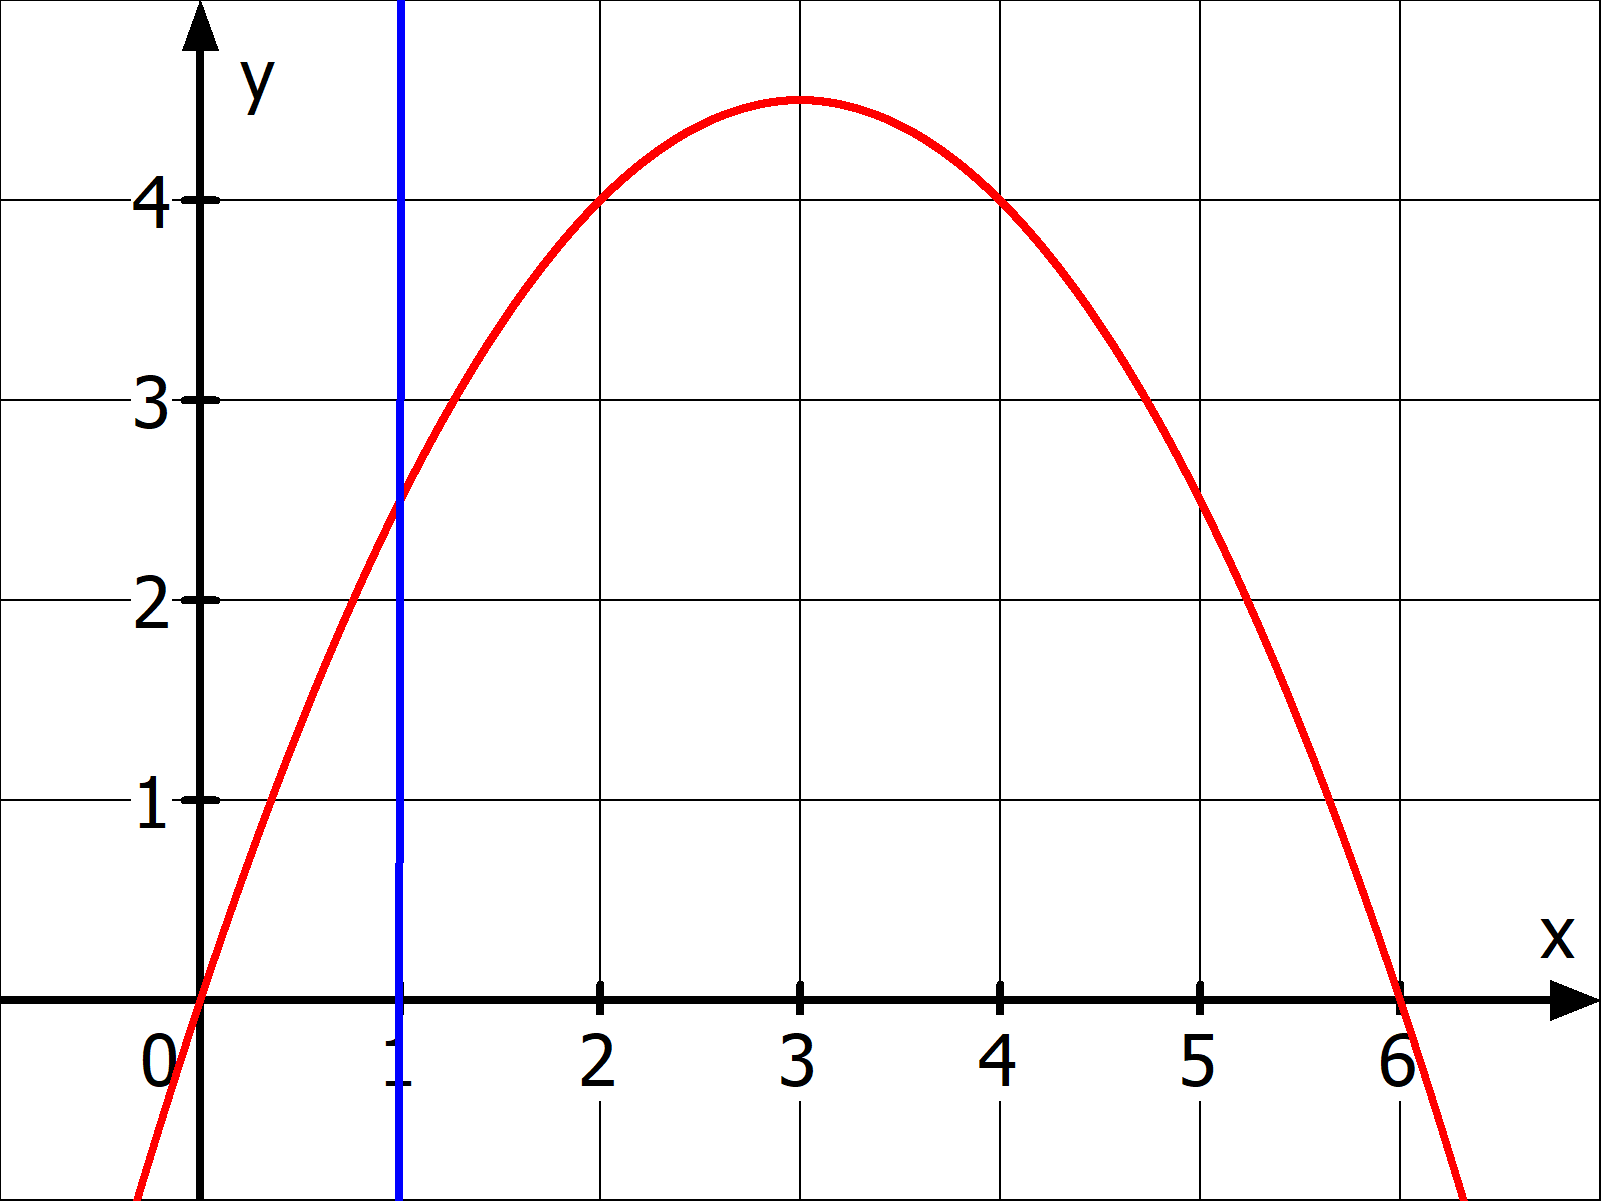
\includegraphics[width=.95\linewidth]{\integration/pics/VerhaeltnisAuf1.png}
		\end{minipage}
		\begin{minipage}{.6\textwidth}\raggedright
			Die zwei Teilflächen lassen sich z.B. wie folgt bestimmen:\\
			Flächeninhalt der linken der beiden Teilflächen:.\\
			\(\displaystyle A_1=\int_{0}^1 -\frac{1}{2}x^2+3x \td x=\frac{4}{3}\)\\
			Flächeninhalt der rechten der beiden Teilflächen:.\\
			\(\displaystyle A_2=-\int_1^6 -\frac{1}{2}x^2+3x \td x=\frac{50}{3}\)\\
			Damit teilt die Gerade \(x=1\) die Fläche zwischen der Funktion und der \(x\)-Achse im Verhältnis \(\dfrac{A_1}{A_2}=\dfrac{2}{25}\).\\
		\end{minipage}
	\end{minipage}
\end{Answer}
\begin{Answer}[ref=verhaltnisFlaechenA2]\\
	\begin{enumerate}[label=\alph*)]
		\item Berechnen der beiden Flächen:
		\begin{align*}
			-\int_{-4}^{-3}\frac{1}{6}x^3+\frac{1}{2}x^2 \td x&=\frac{9}{8}\\
			\int_{-3}^{0}\frac{1}{6}x^3+\frac{1}{2}x^2 \td x&=\frac{9}{8}
		\end{align*}
		Die beiden Flächen haben also beide den gleichen Flächeninhalt von \(\frac{9}{8}\).
		\item Berechnen der beiden Flächen:
		\begin{align*}
			\int_{-3}^{0}\frac{1}{6}x^3+\frac{1}{2}x^2 \td x&=\frac{9}{8}\\		
			\int_{0}^{2}\frac{1}{6}x^3+\frac{1}{2}x^2 \td x&=2
		\end{align*}
		Die beiden Flächen stehen also im Verhältnis \(\dfrac{2}{9/8}=\dfrac{16}{9}\).	
	\end{enumerate}
\end{Answer}
\begin{Answer}[ref=verhaltnisFlaechenA3]\\
	\begin{enumerate}[label=\alph*)]
		\item Berechnen die Fläche \(A\):
		\[A=\int_0^9 -\frac{1}{18}x^3+\frac{1}{2}x^2 \td x=\frac{243}{8}\]
		\item Berechnen der beiden Flächen:\\
		\begin{minipage}{\textwidth}
			\begin{minipage}{.5\textwidth}\raggedright
				\[A_2=\int_3^9 -\frac{1}{18}x^3+\frac{1}{2}x^2-\left(-\frac{1}{2}x+\frac{9}{2}\right) \td x=18\]
				Die Fläche \(A_1\) ergibt sich dann aus
				\[A_1=A-A_2=\frac{243}{8}-18=\frac{99}{8}\]
				Die Gerade teilt die Fläche \(A\) also im Verhältnis \(\dfrac{A_2}{A_1}=\dfrac{18}{99/8}=\dfrac{16}{11}\)
			\end{minipage}
			\begin{minipage}{.5\textwidth}
				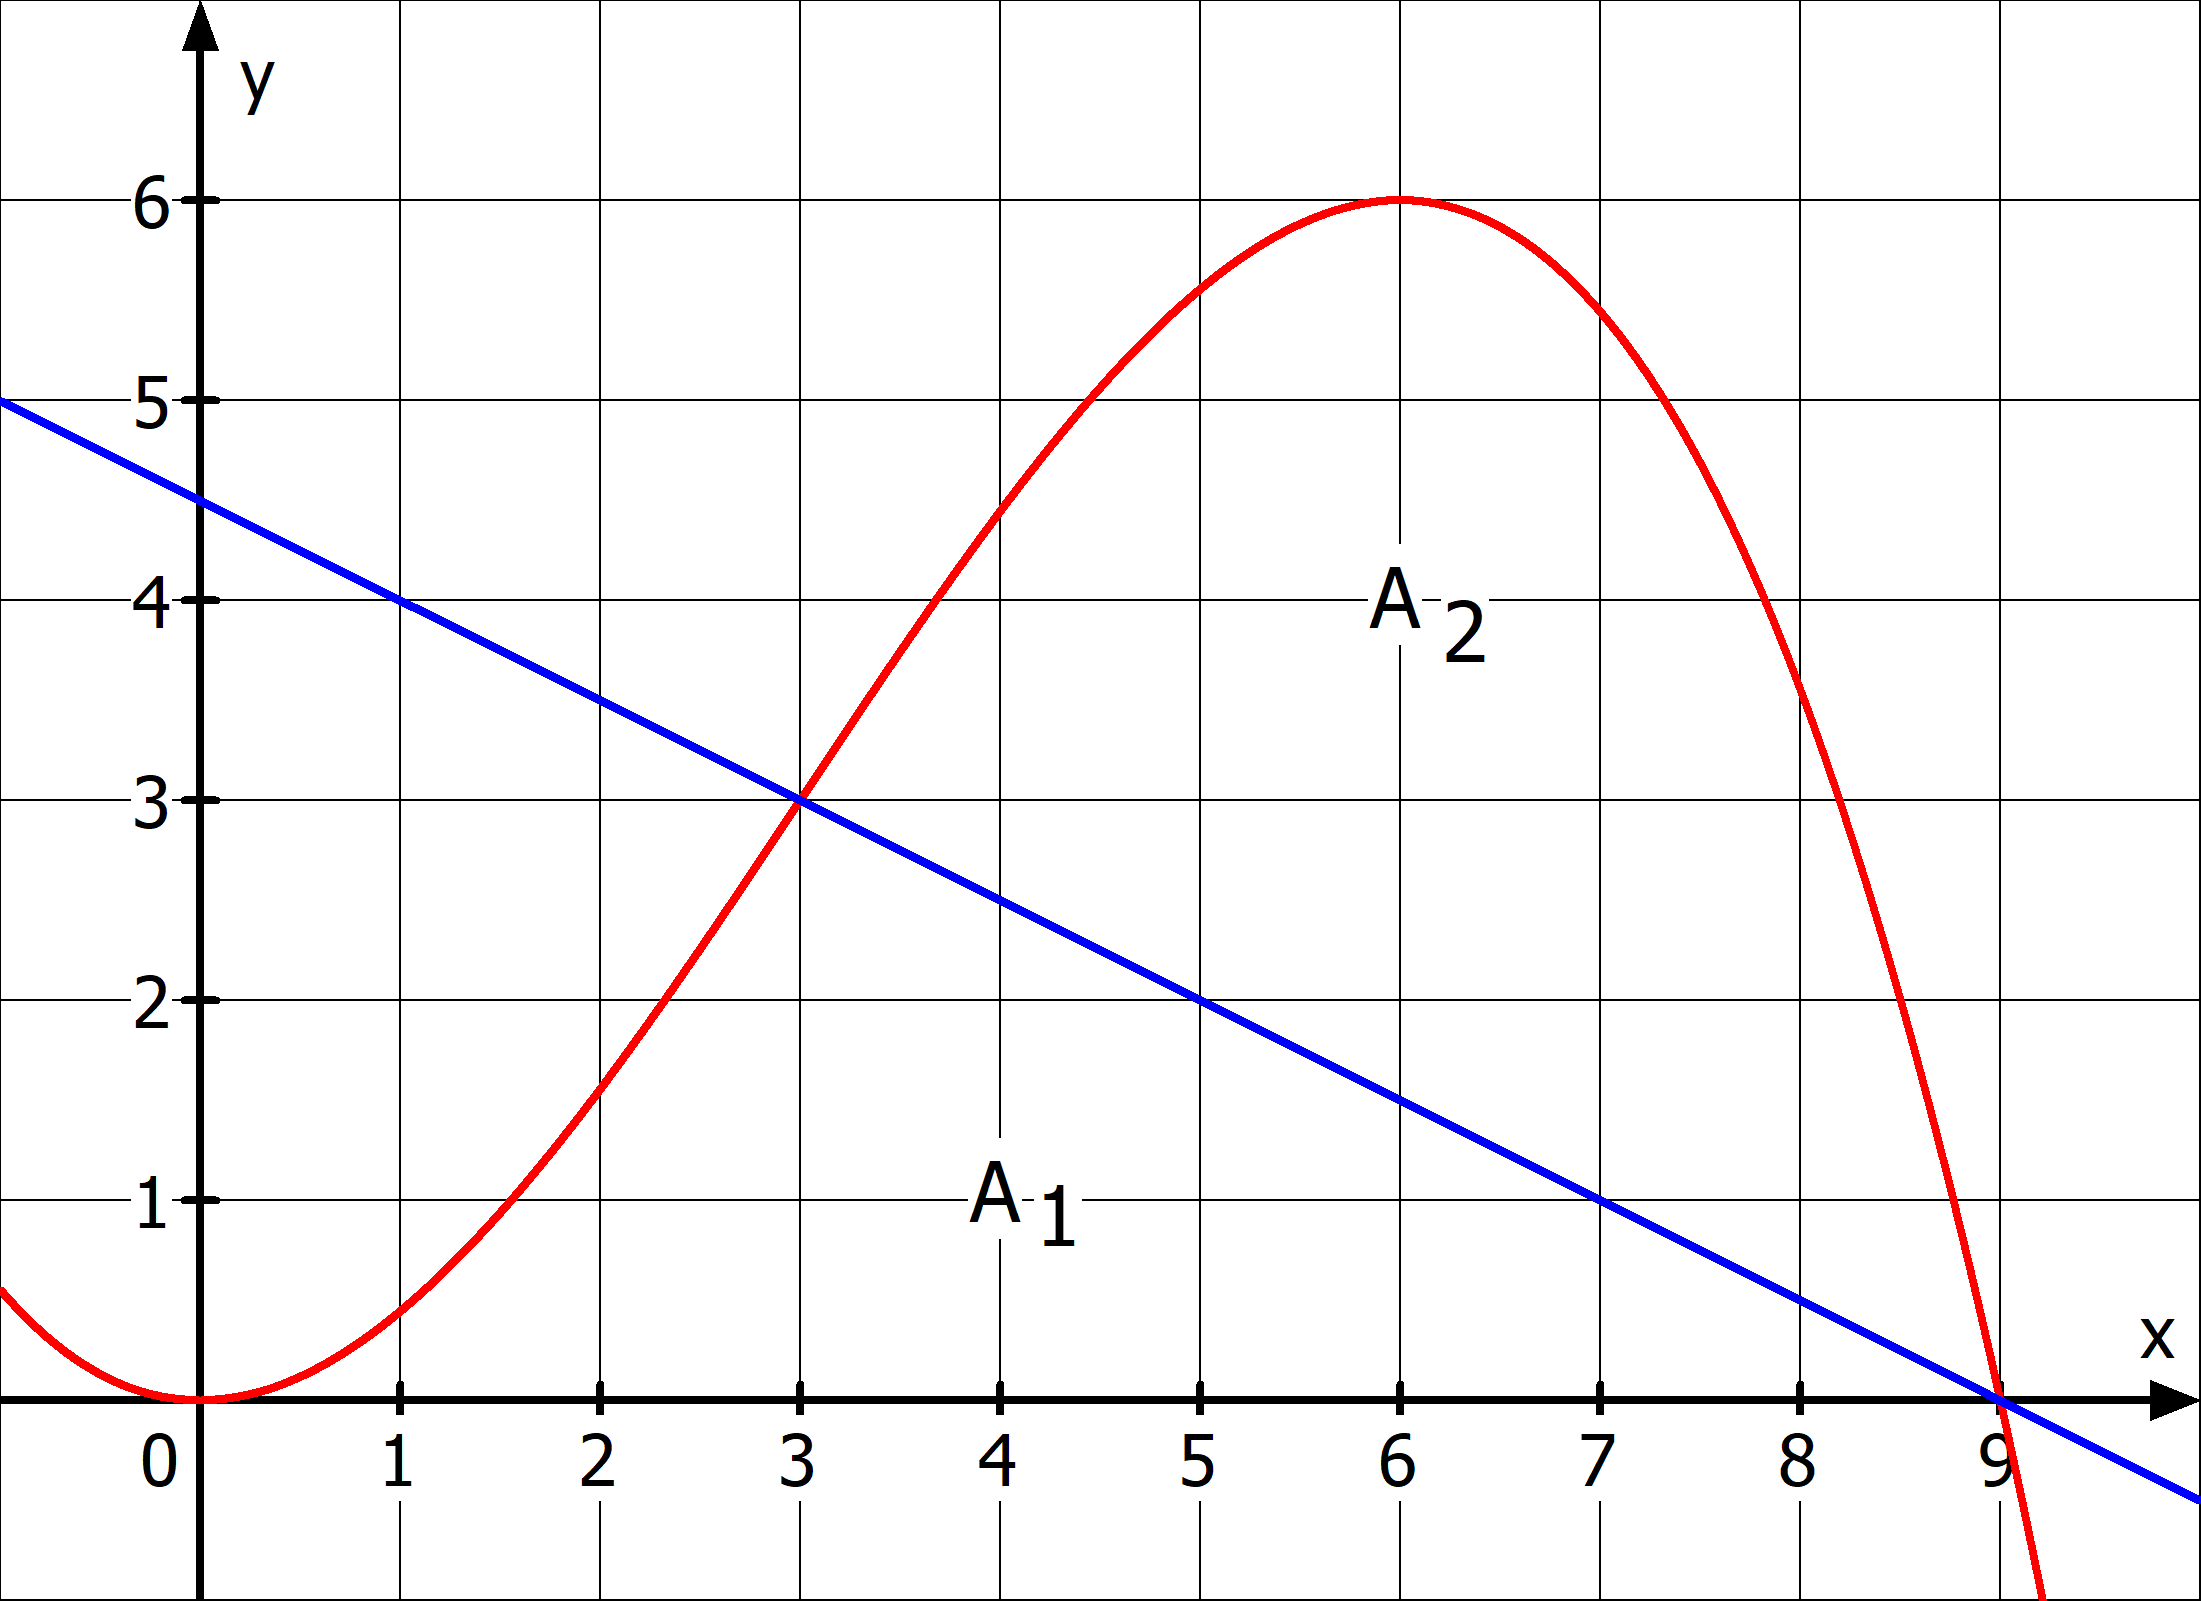
\includegraphics[width=.95\linewidth]{\integration/pics/VerhaeltnisAuf3_Loesung.png}
			\end{minipage}
		\end{minipage}	
	\end{enumerate}
\end{Answer}
%%%%%%%%%%%%%%%%%%%%%%%%%%%%%%%%%%%%%%%%%%
%\newpage
%\cohead{\Large\textbf{Lösungen}}
%\fakesubsection{Lösungen}
%\shipoutAnswer
\end{document}

\begin{enumerate}[label=\alph*)]
\setcounter{enumi}{3}
\item \(a=-1\) und \(b=2\)
\item \(a=-1\) und \(b=1\)
\item \(a=0\) und \(b=2\)
\end{enumerate}


\begin{Exercise}[title={\raggedright xxxxxxxxxxxxxxxxxxxxxxxxx}, label=xxxxxxxxxxxxxxxxxxxx]\\
\begin{minipage}{\textwidth}
	\adjustbox{valign=t}{\begin{minipage}{0.5\linewidth}
			\begin{enumerate}[label=\alph*)]
				\item
			\end{enumerate}
	\end{minipage}}%
	\adjustbox{valign=t}{\begin{minipage}{0.5\linewidth}
			\begin{enumerate}[label=\alph*)]
				\setcounter{enumi}{13}
				\item
			\end{enumerate}
	\end{minipage}}
\end{minipage}
\end{Exercise}
\begin{Answer}[ref=xxxxxxxxxxxxxxxxxxx]\\
\begin{minipage}{\textwidth}
	\adjustbox{valign=t}{\begin{minipage}{0.5\linewidth}
			\begin{enumerate}[label=\alph*)]
				\item
			\end{enumerate}
	\end{minipage}}%
	\adjustbox{valign=t}{\begin{minipage}{0.5\linewidth}
			\begin{enumerate}[label=\alph*)]
				\setcounter{enumi}{13}
				\item
			\end{enumerate}
	\end{minipage}}
\end{minipage}
\end{Answer}